\sectionthree{Complex numbers}
\begin{python0}
from solutions import *; clear() 
\end{python0}

When factoring your characteristic equation, you might get
complex roots.
Here's a quick intro or recap of complex numbers.

A complex number is a number of form
\[
z = a + bi
\]
where $a, b$ are real numbers.
The $i$ is a shorthand for $\sqrt{-1}$.
We say that the real part of $z$ is $a$ and the complex part of $z$ is $b$.
The set of complex numbers include the set of real numbers since
if $a$ is a real number then
\[
a = a + 0i
\]
You can add complex numbers $z = a + bi$ and $z' = a' + b'i$ like this:
\[
z + z' = (a+a') + (b+b')i
\]
For instance $(1+3i) + (0.2 + 1.7i) = 1.2 + 4.7i$. 
You can subtract likewise
\[
z - z' = (a-a') + (b-b')i
\]
You can also multiply complex numbers:
\[
zz' = (a + bi)(a' + b'i) = aa' + ab'i + a'bi + bb'i^2
\]
Note that since $i = \sqrt{-1}$, we have $i^2 = -1$,
\begin{align*}
zz' = aa' + ab'i + a'bi + bb'(-1) = (aa' - bb') + (ab' + a'b)i
\end{align*}

The multiplication of complex numbers seems to be the most complicated.
But the thing to remember is this:
You should not memorize the multiplication formula.
You only need to remember $i^2 = -1$.
In fact a good way to remember everything above is to think of the
$i$ as a variable $X$ and you are sort of like working with
polynomials.
For instance the above then becomes clear:
\[
(a + bX) + (a' + b'X) = (a+a') + (b + b')X
\]
and
\[
(a + bX) (a' + b'X) = (a'b') + (ab' + a'b)X + (bb')X^2
\]
The only thing different between the variable $X$ and $i$ is
that $i^2 = -1$.
Therefore in the above you remember to replace $X$ by $i$ and
$X^2$ by -1.
So remember this: think of $i$ as a variable $X$ except that this
variable has the rule $X^2 = -1$.
Not only that since $X^2 = -1$, you have $X^3 = X^2 \cdot X = -X$,
and $X^4 = X^3 \cdot X = (-X)X = -X^2 = -(-1) = 1$.
In terms of $i$, you have the following integer powers of $i$:
\[
i, \,\,\,\,\,
i^2 = -1, \,\,\,\,\,
i^3 = -i, \,\,\,\,\,
i^4 = 1, 
\]
Of course after that it repeats:
\[
i^5 = i^4 \cdot i, 1 \cdot i = i, \,\,\,\,\,
i^6 = i^4 \cdot i^2, 1 \cdot i^2 = -1, \,\,\,\,\,
\text{etc.}
\]
As you multiply more and more complex numbers you might accumulate
higher and higher powers of $i$.
But remember that you never need more than $i^1$
because all higher powers of $i$ can be rewritten in terms of $\pm i$ or 
$\pm 1$.
In general
\begin{align*}
i^{4n} &= i \\
i^{4n+1} &= i \\
i^{4n+2} &= -1 \\
i^{4n+3} &= -i
\end{align*}
where $n$ is an integer.
(There's no reason to memorize this. 
Just go through the earlier computation of power of $i$ and you'll see it.)
In hifaluting jargon, the integral powers of $i$ has a period of $4$,
just like the sine function has a period of $2\pi$ since
$\sin(x + 2\pi) = \sin(x)$.

Now I need to tell you how to divide complex numbers.
Note that if $z$ and $z'$ are complex numbers, we obviously want $z/z' = z \cdot (1/z')$.
Therefore it's enough for me to tell you how to compute $1/z'$ given $z'$.
If $z' = a' + b'i$ then
\begin{align*}
\frac{1}{z'} 
&= \frac{1}{a' + b'i} \cdot \frac{a' - b'i}{a' - b'i} \\
&= \frac{a' - b'i}{a'^2 + b'^2}
\end{align*}
The key thing to remember about the above is that you're
basically trying to \textit{force the denominator to be a real number}.
And to do that you need to remember that
for any complex number $a' - b'i$, 
\[
(a' - b'i) \cdot (a' + b'i)
\]
will always be a real numbers.
The two complex numbers $a' - b'i$ and $a' + b'i$ are said to be
\textit{complex conjugates}.
This is not as foreign as you think.
If you're experiencing a de jevu, then that's because of examples like 
this (\lq\lq rationalization'') in high school:
\[
\frac{1}{2 + 3 \sqrt{7}} 
\cdot 
\frac{2 - 3\sqrt{7}}{2 - 3\sqrt{7}}
= \frac{2 - 3\sqrt{7}}{2^2 - 9^2 \cdot 7}
\]
So just like multiplying $a' - b' \sqrt{7}$ with $a' + b' \sqrt{7}$
makes the $\sqrt{7}$ go away, multiplying $a' - b'i$ with $a' + b'i$
makes the $i = \sqrt{-1}$ go away.
That's all there is to it.
Note that the method of rationalizing it not specific to $\sqrt{7}$ or
$\sqrt{-1}$. So for an expression of the form $a + b\sqrt{c}$ 
where $a, b, c$ comes from a set of numbers where $\sqrt{c}$ is not in 
this set of numbers, multiplying this number with $a - b\sqrt{c}$
will remove $\sqrt{c}$. 
In the case of $a + b\sqrt{7}$, the set is usually the rationals
which is why you want to get rid of $\sqrt{7}$ by rationalization
since $\sqrt{7}$ is not rational (right?)
For the case of $1 + 2i$, the set is real numbers.
We say that $a + b\sqrt{c}$ and $a - b \sqrt{c}$
are conjugates.

There are two main reasons why we rationalize such expressions.
First it makes computation easier.
Without calculator, an expression like $1/(2 + 3 \sqrt{7})$
would require us to check tables for $\sqrt{7}$, multiply it with $3$ (easy),
add 2 to it (also easy) and then computing the reciprocal, which is
tedious because you're doing division with a number with lots of decimal 
places 
(depending on how accurate you want your number to be).
If you're doing an engineering project and the required accuracy is 10 decimal
places, then your division would be really terrible 
(without a calculator that it.)
So instead of that we rational it to get $\frac{2 - 3\sqrt{7}}{-563}$
Note that this expression is a lot easier to compute without calculators.
You again check the tables for $\sqrt{7}$, multiply it with -3 (easy),
add 2 to it (easy), and divide by $-563$. 
Compare the above two different ways of getting an approximation of 
$1/(2 + 3 \sqrt{7})$.

Another reason why we rationalize is that by doing so,
it changes an expression 
to a standard form that allows us to add, subtract,
and multiply easily. (So again this has to do with easy computation.)
For instance if we want to add $(2 + 3\sqrt{7}) + \frac{1}{2 - 3 \sqrt{7}}$,
you would be forced to approximate the second number if you do not know
how to rationalize it. However with rationalization, you're basically
adding
\begin{align*}
(2 + 3\sqrt{7}) + \biggl( \frac{1}{2 - 3 \sqrt{7}} \biggr)
&=
(2 + 3\sqrt{7}) + \biggl( \frac{2 - 3\sqrt{7}}{-563} \biggr) \\
&=
(2 + 3\sqrt{7}) + \biggl( \frac{2}{-563} - \frac{3}{-563}\sqrt{7} \biggr) \\
&=
\biggl( 2 + \frac{2}{-563} \biggr)
+ \biggl( 3 - \frac{3}{-563} \biggr) \sqrt{7}
\end{align*}
and the above computation is exact.
(Of course if you're only interesting in an approximation
and you have a calculator, rationalizing is redundant.)

\begin{ex}
How do you rationalize $\displaystyle\frac{1}{1 + 2^{1/3}}$? 
(See the \textit{cube} root? It's not a square root.)
\end{ex}

Let's try an example. 
\begin{align*}
\frac{1 + 2i}{3 + 4i}
&= \frac{(1 + 2i)(3 - 4i)}{(3 + 4i)(3 - 4i)} \\
&= \frac{3 - 4i + 6i -8i^2}{3^2 + 4^2} \\
&= \frac{3 +2i + 8}{9 + 16} \\
&= \frac{11 + 2i}{25} \\
&= \frac{11}{25} + \frac{2}{25}i \\
\end{align*}

Let's check that 
\begin{align*}
1 + 2i
&= \biggl( \frac{11}{25} + \frac{2}{25}i \biggr) (3 + 4i)\\
\end{align*}
The right hand side is
\begin{align*}
\biggl( \frac{11}{25} + \frac{2}{25}i \biggr) (3 + 4i)
&= \frac{11}{25} \cdot 3 + \frac{11}{25} \cdot 4i + \frac{2}{25}i \cdot 3 + \frac{2}{25}i \cdot 4i \\
&= \biggl( \frac{11}{25} \cdot 3 -  \frac{2}{25} \cdot 4 \biggr) + \biggl( \frac{11}{25} \cdot 4 + \frac{2}{25} \cdot 3 \biggr)i \\ 
&= \biggl( \frac{33 - 8}{25} \biggr) + \biggl( \frac{44 + 6}{25} \biggr)i \\
&= \biggl( \frac{25}{25} \biggr) + \biggl( \frac{50}{25} \biggr)i 
\end{align*}
which of course does give me $1 + 2i$.

The important thing about the complex numbers is not that it's just a bunch of abstract symbols that we write down.
The important thing is that the complex numbers include the real numbers not just as a set -- 
the operation (addition, subtraction, multiplication, division) on the complex numbers extend the operation on real numbers.
This means for instance that when you look at the above addition of complex numbers you see that
when the complex numbers you're adding are actually real numbers (i.e. their complex parts are actually zero)
then the addition is in fact the addition from real numbers.
For instance the addition formula for complex numbers gives
\[
(3 + 0i) + (2 + 0i) = (3 + 2) + (0 + 0)i = 5 + 0i
\]
which in this case is the same as the addition of \textit{real} numbers
\[
3 + 2 = 5
\]
This is the same for multiplication:
\[
(3 + 0i)(2 + 0i) = (3 \cdot 2 - 0 \cdot 0) + (3 \cdot 0 + 0 \cdot 2) i = (6 - 0) + (0 + 0)i = 6 + 0i
\]
which is just the following multiplication of \textit{real} numbers:
\[
3 \cdot 2 = 6
\]

Now why do we need to extend the real numbers to get the complex numbers?
The reason is that when we have a question regarding real numbers, the question can be viewed as a question regarding
complex numbers.
How so?
Well take for instance look at the equation
\[
x^2 + 1 = 0
\]
viewed as an equation in real numbers, i.e., we want to find real numbers $x$ satisfying
\[
x^2 + 1 = 0
\]
Of course there are no such real numbers!
(One property of real numbers is that $x^2 \geq 0$ for any real number $x$.
Therefore $x^2 + 1 \geq 0 + 1 = 1$.)
However when you view this as an equation in the world of complex numbers, if you like you can write
\[
(1 + 0i)x^2 + (1+0i) = (0 + 0i)
\]
but we usually don't include the complex part of a complex number is it's zero; likewise we leave out the
real part of a complex number when it's 0.
So I'll just write
\[
x^2 + 1 = 0
\]
but remember that all numbers are complex.
Now in this case (i.e., viewing the equation in the complex world), we see that there are now
solutions!!
In fact is $x = i$ (i.e. $\sqrt{-1}$), we get
\[
i^2 + 1 = (-1) + 1 = 0
\]
i.e., in the complex world this equation $x^2 + 1 = 0$ now has solutions!!!
How many solutions are there? Just one?
No, there are two.
The other one is $x = -i$:
\[
(-i)^2 + 1 = (-i)(-i) + 1 = -1 + 1 = 0
\]
(Use the multiplication rule for complex number to compute $(-i)(-i)$.)
Therefore in the real world
\[
x^2 + 1 = 0
\]
has no solutions while in the \textit{complex} world
\[
x^2 + 1 = 0
\]
has two solutions.
In fact there are exactly two solutions.

With complex numbers, any equation involving a quadratic equation
with real coefficients, say 
\[
x^2 + 1 = 0
\] 
will have two roots, i.e. $x = \pm i = \pm \sqrt{-1}$.
But what about
\[
x^2 + 3 = 0
\]
Since we have
\[
x^2 = -3
\]
and hence
\[
x = \pm \sqrt{-3}
\]
do we now need to also add numbers like $\sqrt{-3}$ to our already
expanded real numbers, i.e., complex numbers?
NO! The reason is that
\[
\sqrt{-3} = \sqrt{(-1)(3)} = \sqrt{-1} \cdot \sqrt{3} = 3i
\]
So we do not need to introduce more exotic complex numbers 
\[
\sqrt{-2}, \sqrt{-3}, \sqrt{-1.46}, \ldots
\]
because already in our
complex numbers we can already handle these numbers, which are  
\[
i\sqrt{2}, i\sqrt{3}, i\sqrt{1.46}, \ldots
\]

With $i$ we can now say that the solutions to
\[
ax^2 + bx + c = 0
\]
are
\[
x = \frac{-b \pm \sqrt{b^2 - 4ac}}{2a}
\]
without lawsuits as long as we allow include complex numbers.
(See the square root? The $b^2 - 4ac$ can be negative -- and we
are not worried with that because we have complex numbers.)
Therefore with complex numbers and multiplicity we can say that
every quadratic polynomial has exactly two roots.
We don't have special cases: real distinct roots, one real root, no real
solutions.

Everything is going real well with quadratic polynomials ... but what about 
other polynomials?
Do we need to add some kind of cube root of our complex numbers to 
handle cubic (i.e. degree 3) polynomials?
Take a look at this equation:
\[
x^3 + 1 = 0
\]
i.e.
\[
x^3 = -1
\]
We know that $-11$ is a solution.
Can we add something (some funky super-duper complex numbers) 
to our complex numbers to increase the number of solutions?
Surprisingly there are two solutions not among the real numbers, but which
are in the complex numbers. 
You don't need extra super-duper complex numbers.
Look at this complex number
$z = \frac{1}{2} + \frac{\sqrt{3}}{2}i$.
\[
z^3 = \biggl( \frac{1}{2} + \frac{\sqrt{3}}{2}i \biggr)^3
\]
Now we use binomial theorem to get
\begin{align*}
z^3 
&= \frac{1}{2}^3 + 
3 \biggl( \frac{1}{2} \biggr) ^2 \frac{\sqrt{3}}{2}i + 
3\frac{1}{2} \biggl( \frac{\sqrt{3}}{2}i \biggr)^2 + 
\biggl( \frac{\sqrt{3}}{2}i \biggr)^3\\
\end{align*}
Looks bad ... but it's just a tedious computation.
Let me do it slowly.
\begin{align*}
z^3 
&= \frac{1}{8}
\biggl(
1 + 
3 \sqrt{3}i + 
3 (\sqrt{3}i)^2 + 
(\sqrt{3}i)^3
\biggr) \\
&= \frac{1}{8}
\biggl(
1 + 
3 \sqrt{3}i + 
3 \cdot \sqrt{3}^2 i^2 + 
\sqrt{3}^3 i^3
\biggr)
\\
&= \frac{1}{8}
\biggl(
1 + 
3 \sqrt{3}i + 
9 i^2 + 
3 \sqrt{3} i^3
\biggr)
\\
\end{align*}
Now we lower the powers of $i$ in the expression:
\begin{align*}
z^3 
&= \frac{1}{8}
\biggl(
1 + 
3 \sqrt{3}i + 
9 (-1) + 
3 \sqrt{3} (-i)
\biggr)
\end{align*}
Now you see that some terms combine:
\begin{align*}
z^3 
&= \frac{1}{8}
\biggl(
(1 + 9(-1))+ 
(3 \sqrt{3}i +  3 \sqrt{3} (-i))
\biggr) \\
&= \frac{1}{8} (-8 + 0) \\
&= -1
\end{align*}
V\'oila!

\begin{ex}
  The above is an exponentiation computation on
  a complex number.
  The above computation uses binomial theorem.
  Later you'll learn the 
  de Moivre's theorem, a very powerful tool for exponentiation.
  After you learn de Moivre's theorem, come back to this problem
  and compute
  $\left(\frac{1}{2} + \frac{\sqrt{3}}{2}i \right)^3$
  using de Moivre's theorem.
  \qed
\end{ex}

It's curious that a cubic polynomial can have extra roots
just like the quadratic polynomial simply because we've 
\lq\lq repaired'' the real numbers just by handling only 
the quadratic case.

But are there any other solutions? 

\begin{ex}
Your turn ... show that 
\[
z' = \frac{1}{2} - \frac{\sqrt{3}}{2}i
\] 
is another
solution to $x^3 = -1$.
\end{ex}

It turns out that the $i$, which is inherently a creature of the 
\textit{square root},
is actually enough to solution \textit{every} polynomial,
cubic, quartic (degree 4), quintic (degree 5), sextic (degree 6), 
whatever-tic.

In fact in the complex world any polynomial of degree $d$ has \textit{exactly} $d$
roots. 
You have to be careful here with how you count roots.
For instance
\[
(x - 1)^2 = 0
\]
has two roots (or we say that root 1 occurs with multiplicity of 2.)
In order words you  can't just find some number $a$ and say that 
$a$ is a root of polynomial $p(x)$ simply because $p(a) = 0$, and happy
go on the the next number. Once you've found a root say $a$
you need to factor out as many $x-a$'s from 
your polynomial as you can to get $p(x) = (x-a)^n q(x)$
such that $q(a) \neq 0$ 
then conclude that $a$ occurs $n$ times (or we say it has multiplicity $n$,
then find other numbers for satisfying $q(x) = 0$, etc., until you get
something like
\[
p(x) = c(x-a)^n (x-b)^m ...
\]
then you say that you've found all the roots, i.e. $a$ occurs $n$ times, $b$ occurs
$m$ times, etc. 

The big theorem regarding complex numbers is that you can \textit{always} find a complex
root for your polynomial $p(x)$ as long as the degree is $\geq 1$ and with that
root, say $a$, you can factorize $p(x)$ as $(x-a)^nq(x)$.
You then repeat the process with $q(x)$ to get $q(x) = (x-b)^m r(x)$, and hence
$p(x) = (x-a)^n(x-b)^m r(x)$, etc., until you've found all the roots.
The other part of this big theorem is that not can you \textit{always} find a root,
the number of roots (again counting repeats) will \textit{always} be the degree
of the polynomial.

This is called the fundamental theorem of algebra.
Once again this says that any polynomial of degree $d$ viewed as a polynomial in complex
numbers will always have exactly $d$ roots.

Another important thing about the factorization of your polynomial $p(x)$ into
something like $c(x-a)^n(x-b)^m \cdots$ is that the factorization is unique.
OK what do I mean by that?
Well suppose instead factorizing it \lq\lq root by root, what if you 
manage to factor a degree 100 polynomial into two with degree 40 and 60?
say $p(x) = u(x) v(x)$.
If you carry out the factorization on $u(x)$ and $v(x)$, you will
still get them into the form $c_1(x-a_1)^{n_1} \cdots$ and $c_2(x-a_2)^{n_2} \cdots$.
Putting these back into $p(x) = c_1(x-a_1)^{n-1} \cdots c_2(x-a_2)^{n_2} \cdots$,
you'll find that the linear terms, i.e., the $x-\alpha$ terms that appear will always
be the same, it doesn't matter how you carry out the factorization.
Again, once you finish factorization into linear terms, you get the same thing.

This is similar to the integers.
For instance look at the number 100.
If you factorize it by factoring out the smallest primes, you can
the following:
\[
100 = 2 \cdot 50 = 2 \cdot 2 \cdot 25 = 2 \cdot 2 \cdot 5 \cdot 5
\]
If however you factorize it by break off a 10 first:
\[
100 = 10 \cdot 10
\]
and then factorize the 10's separately to get $10 = 2 \cdot 5$ and then 
put everything together to get:
\[
100 = 10 \cdot 10 = 2 \cdot 5 \cdot 2 \cdot 5
\]
you see the the \lq\lq smallest'' nontrivial factors
(i.e. primes), i.e. 2, 2, 5, 5, are the same
in both cases.
If you prefer a picture here's one:
\begin{verbatim}
      100                 100
     /   \               /   \
    2    50             10   10
        /  \           /  \ /  \
       2   25          2  5 2  5
          /  \
         5    5
\end{verbatim}

The analogy is more than a mere curiosity. 
There is a deep connection between the math of integers and the
math of polynomials.

By the way the corresponding theorem for integer is called
the fundamental theorem of arithmetic.
So you have now seen:
\begin{enumerate}[nosep]
\li The fundamental theorem of arithmetic
\li The fundamental theorem of algebra
\end{enumerate}

Let's go back to computations.
I've given you the solutions to $x^3 + 1 = 0$.
But ...
how did I come up with the solutions
\[
z = \frac{1}{2} + \frac{\sqrt{3}}{2}i
\]
and
\[
z' = \frac{1}{2} - \frac{\sqrt{3}}{2}i
\] 
for $x^3 = -1$?!?
Furthermore ... something's fishy here ...
$z,z'$ are conjugates.

First of all, note that the fundamental theory of algebra is useful
because it tells us that $x^3 + 1$ has 3 roots.
So at least we know that together with $-1$ there are no other roots:
the fundamental theorem of algebra tells us when we can stop the search for
roots.
But it doesn't tell us how to find the roots!

Here's where trigonometry and geometry come to the rescue!

First you can draw complex numbers on a 2-D plane called the complex
plane:
%-*-latex-*-

\begin{center}
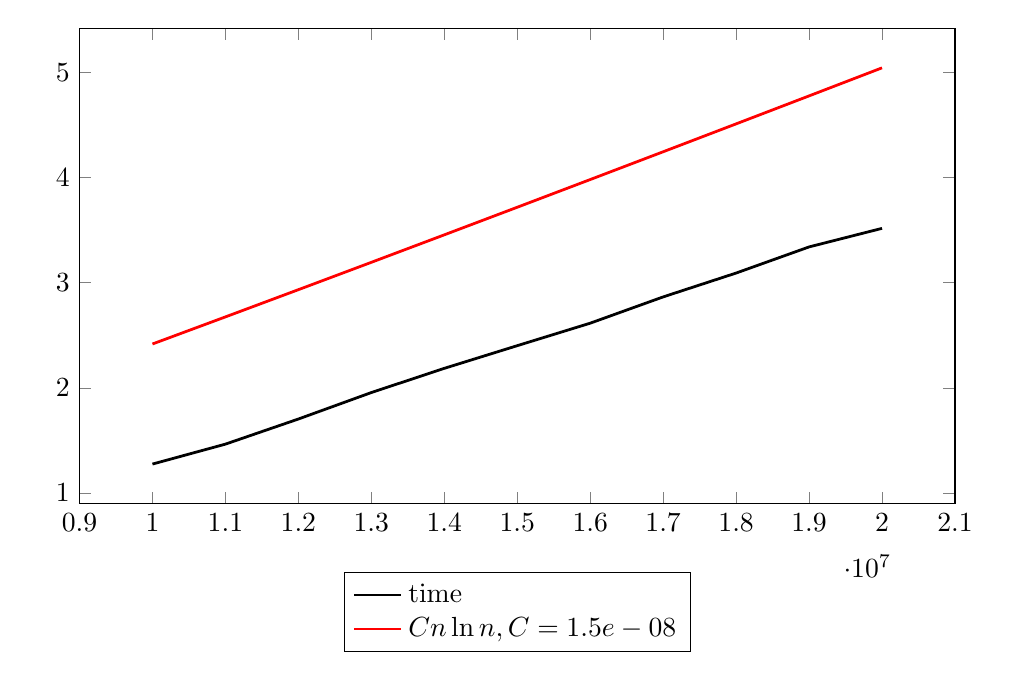
\begin{tikzpicture}[line width=1]
\begin{axis}[width=5in, height=3in,
             scatter/classes={a={mark=*,draw=black}},
             xlabel={\mbox{}},
             xlabel style={name=xlabel}, 
             ylabel={\mbox{}}, 
             legend style={
                at={(xlabel.south)},
                yshift=-1ex,
                anchor=north,
                legend cell align=left,
                },
        ]
]
\addplot[draw=black, line width=1] coordinates {(10000000, 1.27583)
(11000000, 1.46545)
(12000000, 1.70418)
(13000000, 1.9559)
(14000000, 2.18601)
(15000000, 2.40166)
(16000000, 2.6155)
(17000000, 2.86536)
(18000000, 3.0922)
(19000000, 3.34059)
(20000000, 3.51714)};\addlegendentry{time}\addplot[draw=red, line width=1] coordinates {(10000000, 2.4177143476437477)
(11000000, 2.6752119620758363)
(12000000, 2.934075097395409)
(13000000, 3.1941896835080326)
(14000000, 3.4554592563917015)
(15000000, 3.7178011707899588)
(16000000, 3.981143827248973)
(17000000, 4.2454245950152245)
(18000000, 4.510588225282318)
(19000000, 4.776585618082254)
(20000000, 5.043372849455478)};\addlegendentry{$C n \ln n, C =1.5e-08$}
\end{axis}\end{tikzpicture}\end{center}

For instance here's $1 + 2i$:
\input{plot1.tex}
Note in particular that real numbers are entirely on the real axis.
For instance here's $\pi = 3.14159...$ approximately:
\input{plot2.tex}
Here's $i$:
\input{plot3.tex}
In general $a + bi$ is at the point $(a,b)$ of the 2-D plane.
\input{plot4.tex}

Now I'm going to put our solutions of $x^3 + 1 = 0$ into the complex
plane:
\input{plot5.tex}

Now I'm going to draw lines from 0 to the roots:
\begin{center}
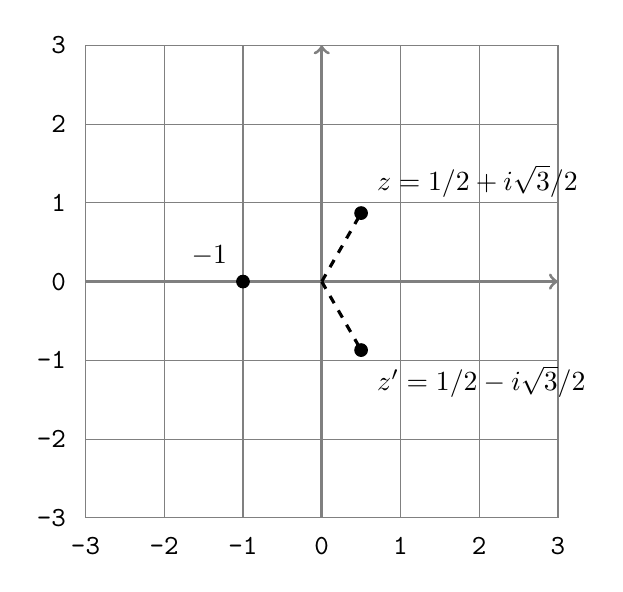
\begin{tikzpicture}
\draw[gray] (-3,-3) to  (-3,3);
\draw[gray] (-2,-3) to  (-2,3);
\draw[gray] (-1,-3) to  (-1,3);
\draw[gray] (0,-3) to  (0,3);
\draw[gray] (1,-3) to  (1,3);
\draw[gray] (2,-3) to  (2,3);
\draw[gray] (3,-3) to  (3,3);
\draw[gray] (-3,-3) to  (3,-3);
\draw[gray] (-3,-2) to  (3,-2);
\draw[gray] (-3,-1) to  (3,-1);
\draw[gray] (-3,0) to  (3,0);
\draw[gray] (-3,1) to  (3,1);
\draw[gray] (-3,2) to  (3,2);
\draw[gray] (-3,3) to  (3,3);
\draw(-3, -3) node [font=\ttfamily, label=below:{\normalsize {\texttt{-3}}}] {};
\draw(-2, -3) node [font=\ttfamily, label=below:{\normalsize {\texttt{-2}}}] {};
\draw(-1, -3) node [font=\ttfamily, label=below:{\normalsize {\texttt{-1}}}] {};
\draw(0, -3) node [font=\ttfamily, label=below:{\normalsize {\texttt{0}}}] {};
\draw(1, -3) node [font=\ttfamily, label=below:{\normalsize {\texttt{1}}}] {};
\draw(2, -3) node [font=\ttfamily, label=below:{\normalsize {\texttt{2}}}] {};
\draw(3, -3) node [font=\ttfamily, label=below:{\normalsize {\texttt{3}}}] {};
\draw(-3, -3) node [font=\ttfamily, label=left:{\normalsize {\texttt{-3}}}] {};
\draw(-3, -2) node [font=\ttfamily, label=left:{\normalsize {\texttt{-2}}}] {};
\draw(-3, -1) node [font=\ttfamily, label=left:{\normalsize {\texttt{-1}}}] {};
\draw(-3, 0) node [font=\ttfamily, label=left:{\normalsize {\texttt{0}}}] {};
\draw(-3, 1) node [font=\ttfamily, label=left:{\normalsize {\texttt{1}}}] {};
\draw(-3, 2) node [font=\ttfamily, label=left:{\normalsize {\texttt{2}}}] {};
\draw(-3, 3) node [font=\ttfamily, label=left:{\normalsize {\texttt{3}}}] {};
\draw[line width=0.04cm,black!50,->] (-3,0) to  (3,0);
\draw[line width=0.04cm,black!50,->] (0,-3) to  (0,3);

\fill[black] (0.5, 0.87) circle (0.08);
\draw[black] (0.5, 0.87) circle (0.08);
\node[anchor=south west] at (0.58,0.946)   {$z = 1/2 + i\sqrt{3}/2$};

\fill[black] (-1.0, 0.0) circle (0.08);
\draw[black] (-1.0, 0.0) circle (0.08);
\node[anchor=south east] at (-1.08,0.08)   {$-1$};

\fill[black] (0.5, -0.87) circle (0.08);
\draw[black] (0.5, -0.87) circle (0.08);
\node[anchor=north west] at (0.58,-0.946)   {$z' = 1/2 - i\sqrt{3}/2$};
\draw[line width=0.04cm,black,,dashed] (0,0) to  (0.5,0.87);
\draw[line width=0.04cm,black,,dashed] (0,0) to  (0.5,-0.87);
\end{tikzpicture}

\end{center}


There's a very high level of symmetric here!!!
The real axis is like a mirror, reflecting $z$ to get $z'$ 
and vice versa.
It's not just something curious about $z$ and $z'$.
In fact there's something about \textit{all} three solutions:
they are all on a circle of radius 1 about center 0!
\input{plot7.tex}
For instance to show that $z = 1/2 + \sqrt{3}/2 i$ is on a circle
of radius 1, you only need to show that the distance from 0 to $z$
in the above picture is 1.
For that we can use Pythagorus theorem on this triangle
to compute the distance from 0 to $z$ which I'm marking as $r$:
\begin{center}
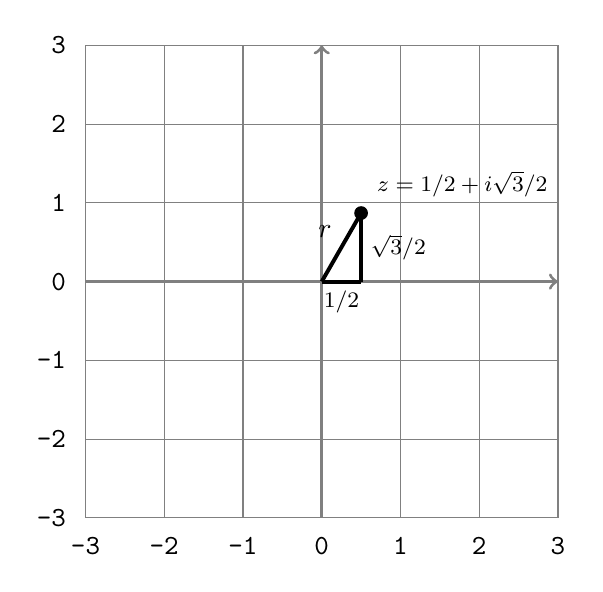
\begin{tikzpicture}
\draw[gray] (-3,-3) to  (-3,3);
\draw[gray] (-2,-3) to  (-2,3);
\draw[gray] (-1,-3) to  (-1,3);
\draw[gray] (0,-3) to  (0,3);
\draw[gray] (1,-3) to  (1,3);
\draw[gray] (2,-3) to  (2,3);
\draw[gray] (3,-3) to  (3,3);
\draw[gray] (-3,-3) to  (3,-3);
\draw[gray] (-3,-2) to  (3,-2);
\draw[gray] (-3,-1) to  (3,-1);
\draw[gray] (-3,0) to  (3,0);
\draw[gray] (-3,1) to  (3,1);
\draw[gray] (-3,2) to  (3,2);
\draw[gray] (-3,3) to  (3,3);
\draw(-3, -3) node [font=\ttfamily, label=below:{\normalsize {\texttt{-3}}}] {};
\draw(-2, -3) node [font=\ttfamily, label=below:{\normalsize {\texttt{-2}}}] {};
\draw(-1, -3) node [font=\ttfamily, label=below:{\normalsize {\texttt{-1}}}] {};
\draw(0, -3) node [font=\ttfamily, label=below:{\normalsize {\texttt{0}}}] {};
\draw(1, -3) node [font=\ttfamily, label=below:{\normalsize {\texttt{1}}}] {};
\draw(2, -3) node [font=\ttfamily, label=below:{\normalsize {\texttt{2}}}] {};
\draw(3, -3) node [font=\ttfamily, label=below:{\normalsize {\texttt{3}}}] {};
\draw(-3, -3) node [font=\ttfamily, label=left:{\normalsize {\texttt{-3}}}] {};
\draw(-3, -2) node [font=\ttfamily, label=left:{\normalsize {\texttt{-2}}}] {};
\draw(-3, -1) node [font=\ttfamily, label=left:{\normalsize {\texttt{-1}}}] {};
\draw(-3, 0) node [font=\ttfamily, label=left:{\normalsize {\texttt{0}}}] {};
\draw(-3, 1) node [font=\ttfamily, label=left:{\normalsize {\texttt{1}}}] {};
\draw(-3, 2) node [font=\ttfamily, label=left:{\normalsize {\texttt{2}}}] {};
\draw(-3, 3) node [font=\ttfamily, label=left:{\normalsize {\texttt{3}}}] {};
\draw[line width=0.04cm,black!50,->] (-3,0) to  (3,0);
\draw[line width=0.04cm,black!50,->] (0,-3) to  (0,3);

\fill[black] (0.5, 0.87) circle (0.08);
\draw[black] (0.5, 0.87) circle (0.08);
\node[anchor=south west] at (0.58,0.946)   {\footnotesize{$z = 1/2 + i\sqrt{3}/2$}};
\draw[line width=0.05cm,black] (0,0) to  (0.5,0.87);

\node[anchor=south east] at (0.25,0.435)   {$\footnotesize{r}$};
\draw[line width=0.05cm,black] (0,0) to  (0.5,0);

\node[anchor=north] at (0.25,0)   {\footnotesize{1/2}};
\draw[line width=0.05cm,black] (0.5,0) to  (0.5,0.87);

\node[anchor=west] at (0.5,0.433)   {\footnotesize{$\sqrt{3}/2$}};
\end{tikzpicture}

\end{center}


With the help of Mr Pythagorus we have:
\[
r = \sqrt{\biggl( \frac{1}{2} \biggr)^2 + \biggl( \frac{\sqrt{3}}{2} \biggr)^2}
= \sqrt{\frac{1}{4} + \frac{3}{4}} = 1
\]


\begin{ex}
Show that $z'$ is also on the circle of radius 1 and center 0.
\end{ex}


Furthermore, the three lines from 0 to the roots divide up the
circle into three equal parts.
In other words the angles between the three lines are exactly 
$360/3 = 120$ degrees.
Why?
Let's look at the above picture again.
The angle  $z$ makes with the real axis is marked $t$:
\begin{center}
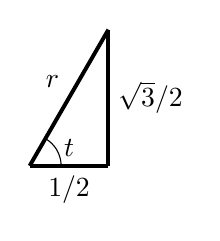
\begin{tikzpicture}
\draw[line width=0.05cm,black] (0,0) to  (1.0,1.73);

\node[anchor=south east] at (0.5,0.865)   {${r}$};
\draw[line width=0.05cm,black] (0,0) to  (1.0,0);

\node[anchor=north] at (0.5,0)   {{1/2}};
\draw[line width=0.05cm,black] (1.0,0) to  (1.0,1.73);

\node[anchor=west] at (1.0,0.866)   {{$\sqrt{3}/2$}};
\draw[] (0.4,0) arc (0:60:0.4);
\node[anchor=south] at (0.5,0)   {{$t$}};
\end{tikzpicture}

\end{center}


From trigo you know that
\[
\tan t = \frac{\sqrt{3}/2}{1/2} = \sqrt{3}
\]
and since this angle is acute (between 0 and 90 degrees)
we see that
\[
t = 60^\circ
\]
which in radians is
\[
t = 60 \cdot \frac{\pi}{180} = \frac{\pi}{3}
\]
I'll let you check that all the three angles are  indeed the same
(in fact they are 120 degrees).

I won't talk about solving the general polynomials for roots.
(In fact it's a difficult subject.)
But there's something that's very useful about describing
complex numbers in terms of it's distance from 0 and the angle it makes
with the positive real axis.

Suppose you have a complex number $z$ and you draw it on the 
complex plane and you've already computed it's distance
from 0, which I will write as $r$, and the angle
it makes with the positive real axis, which I will call $t$:
\begin{center}
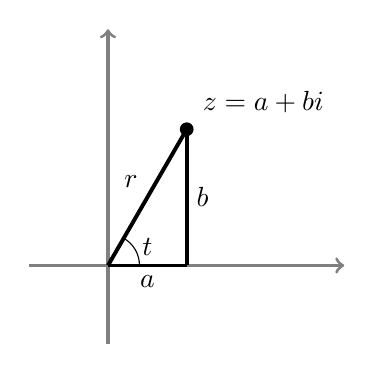
\begin{tikzpicture}
\draw[line width=0.04cm,black!50,->] (-1,0) to  (3,0);
\draw[line width=0.04cm,black!50,->] (0,-1) to  (0,3);

\fill[black] (1.0, 1.73) circle (0.08);
\draw[black] (1.0, 1.73) circle (0.08);
\node[anchor=south west] at (1.08,1.812)   {$z = a + bi$};
\draw[line width=0.05cm,black] (0,0) to  (1.0,1.73);

\node[anchor=south east] at (0.5,0.865)   {${r}$};
\draw[line width=0.05cm,black] (0,0) to  (1.0,0);

\node[anchor=north] at (0.5,0)   {$a$};
\draw[line width=0.05cm,black] (1.0,0) to  (1.0,1.73);

\node[anchor=west] at (1.0,0.866)   {$b$};
\draw[] (0.4,0) arc (0:60:0.4);
\node[anchor=south] at (0.5,0)   {{$t$}};
\end{tikzpicture}

\end{center}


then from trigo you know that, if $z = a + bi$,
\begin{align*}
a &= r \cos t \\
b &= r \sin t 
\end{align*}
In other words
\begin{align*}
z 
&= (r \cos t) + i (\sin t) \\
&= r(\cos t + i \sin t) 
\end{align*}
The complex number 
\[
\cos t + i \sin t
\]
has length 1 from 0.
When written this way
\[
z = (r \cos t) + i (\sin t) \\
\]
we say that $z$ is written in
\defone{polar coordinates}.
When we write $z$ as
\[
z = a + bi
\]
we say that $z$ is written in \defone{rectangle coordinates}.
\begin{prop}
  If $z = a + bi$, then
  \[
  z = r(\cos t + i \sin t)
  \]
  where
  \begin{align*}
    r &= \sqrt{x^2 + y^2} \\
    \tan t &= \frac{b}{a}
  \end{align*}
  \qed
\end{prop}

So what?

There's something special about taking powers of a complex
number written in polar coordinates.
First of all, focusing only on the 
\[
\cos t + i \sin t
\]
\href{https://en.wikipedia.org/wiki/Abraham_de_Moivre}{de Moivre}'s theorem says that

\begin{thm} \textnormal{(\defone{de Moivre's theorem})}
\[
(\cos t + i \sin t)^n
=
\cos (nt) + i \sin (nt)
\]
\end{thm}

When applied to $z$ it means that we have a very fast method for computing
powers:
\begin{align*}
z^n  
&= (r (\cos t + i \sin t))^n \\
&= r^n (\cos (nt) + i \sin (nt))
\end{align*}


\begin{ex}
Compute $(1 + \sqrt{3}i)^{100}$ in two different ways:
\begin{enumerate}[nosep,label=(\alph*)]
\item Use binomial theorem and then simplify.
\item Find $r$ and $t$ such that 
$z = r(\cos t + i \sin t)$. Compute $z^{100}$ using de Moivre's theorem.
\end{enumerate}
\qed
\end{ex}

Here's another thing you can do with de Moivre's theorem.
Remember those pesky trigo identities involving multiple angles?
For instance here are two double angle formulas:
\begin{align*}
  \cos 2x &= \cos^2 x - \sin^2 x \\
  \sin(2x) &= 2 \sin x \cos x
\end{align*}
Here's one way of remember it.
By de Moivre's theorem
\[
(\cos x + i \sin x)^2 = \cos (2x) + i \sin (2x)
\]
But by the binomial theorem
\begin{align*}
(\cos x + i \sin x)^2 
&= (\cos x)^2 + 2 (\cos x)(i \sin x) + (i \sin x)^2 \\
&= \cos^2 x + 2 (\cos x)(i \sin x) + - \sin^2 x \\
&= \cos^2 x + 2 (\cos x)(i \sin x) - \sin^2 x \\
&= (\cos^2 x - \sin^2 x) + 2 i \cos x \sin x
\end{align*}
This means that
\[
\cos (2x) + i \sin (2x)
= (\cos^2 x - \sin^2 x) + 2 i \cos x \sin x 
\]
Now on comparing the real and complex part of the equation you get
\begin{align*}
\cos 2x &= \cos^2 x - \sin^2 x \\
\sin 2x &= 2 \sin x \cos x 
\end{align*}
Tada!
All you need it binomial theorem and de Moivre's theorem
to remember the double angle formula for sine and cosine.

Of course if you just want the formula for $\sin 2x$ you can 
just ignore the real part of the equation.
You can even do this quickly in your head:
\begin{align*}
(...) + i \sin 2x 
&= (\cos x + i \sin x)^2 \\
&= (...) + 2 \cos x i \sin x
\end{align*}
i.e.
\[
\sin 2x = 2 \sin x \cos x
\]

Now let me derive the formulas for $\cos 3x$
again using binomial theorem and de Moivre's theorem:
\begin{align*}
\cos 3x + i \sin 3x
&= (\cos x + i \sin x)^3 \\
&= (\cos x + i \sin x)^3 \\
&= \cos^3 x + (...) + 3\cos^1 x (i\sin x)^2 + (...)
\end{align*}
(ignore the complex part -- do you see why the second and fourth
terms are complex?)
i.e.
\[
\cos 3x = \cos^3 x - 3\cos x \sin^2 x
\]
now use Pythagorus' theorem to convert $\sin^2 x$ to $\cos x$
\[
\sin^2 x + \cos^2 x = 1
\]
and you'll get
\begin{align*}
\cos 3x
&= \cos^3 x - 3\cos x (1-\cos^2 x) \\
&= 4\cos^3 x - 3 \cos x
\end{align*}

\begin{ex}
  Derive $\sin 3x$ in terms of $\sin x$.
  \qed
\end{ex}

I can even do $\cos 4x$ without too much pain:
\begin{align*}
\cos 4x 
&= (\cos x)^4 + 6(\cos x)^2(i\sin x)^2 + (i\sin x)^4 \\
&= \cos^4 x - 6\cos^2 x\sin^2 x + \sin^4 x \\
&= \cos^4 x - 6\cos^2 x(1 - \cos^2 x) + (1 - \cos^2 x)^2 \\
&= 7\cos^4 x - 6\cos^2 x + (1 - 2\cos^2 x + \cos^4 x) \\
&= 8\cos^4 x - 8 \cos^2 x + 1 \\
\end{align*}

\begin{ex}
Your turn ... derive $\sin 4x$ in terms of $\sin x$.
\end{ex}

\begin{ex}
  Factorize $x^2 = 1$ using de Moivre's theorem.
  (Of course you know that the roots are $1, -1$.
  Just pretend you don't.
  Let $z = r (\cos t + i \sin t)$ be a complex
  number satisfying $x^2 = 1$.
  Use de Moivre's theorem and solve for $r$ and $t$.)
  \qed
\end{ex}

\begin{ex}
  Factorize $x^2 = -1$ using de Moivre's theorem.
  \qed
\end{ex}

\begin{ex}
  Factorize $x^3 = 1$ using de Moivre's theorem, i.e.,
  find all the roots of $x^3 = 1$.
  \qed
\end{ex}

\begin{ex}
  Factorize $x^3 = 4$.
  (Use previous exercise.)
  \qed
\end{ex}

\begin{ex}
  Factorize $x^4 = 1$.
  \qed
\end{ex}

\begin{ex}
  Factorize $x^n = 1$ where $n$ is a positive integer.
  \qed
\end{ex}

\newpage
\subsection*{Solutions}

\newpage
\section*{Solutions}
Solution to Exercise \ref{ex:dfa0}\labeltext{}{sol:dfa0}.

\tinysidebar{\debug{exercises/{dfa0/answer.tex}}}

    Solution not provided.
    

\newpage

Solution to Exercise \ref{ex:dfa1}\labeltext{}{sol:dfa1}.

\tinysidebar{\debug{exercises/{dfa1/answer.tex}}}
  The ID computation is
  \begin{align*}
    (q_0, aba)
    &\vdash (\delta(q_0, a), ba) = (q_0, ba) \\ 
    &\vdash (\delta(q_0, b), a) = (q_1, a) \\
    &\vdash (\delta(q_1, a), \ep) = (q_0, \ep)
  \end{align*}
  $q_0$ is not an accept state. Therefore $aba$ is not accepted.


\newpage

Solution to Exercise \ref{ex:dfa4}\labeltext{}{sol:dfa4}.

\tinysidebar{\debug{exercises/{dfa4/answer.tex}}}

    Solution not provided.
    

\newpage

Solution to Exercise \ref{ex:dfa5}\labeltext{}{sol:dfa5}.

\tinysidebar{\debug{exercises/{dfa5/answer.tex}}}

    Solution not provided.
    

\newpage

Solution to Exercise \ref{ex:implementing-a-single-dfa0}\labeltext{}{sol:implementing-a-single-dfa0}.

\tinysidebar{\debug{exercises/{implementing-a-single-dfa0/answer.tex}}}

    Solution not provided.
    

\newpage

Solution to Exercise \ref{ex:nfastatediag0}\labeltext{}{sol:nfastatediag0}.

\tinysidebar{\debug{exercises/{nfastatediag0/answer.tex}}}

    Solution not provided.
    

\newpage

Solution to Exercise \ref{ex:nfastatediag1}\labeltext{}{sol:nfastatediag1}.

\tinysidebar{\debug{exercises/{nfastatediag1/answer.tex}}}

    Solution not provided.
    

\newpage

Solution to Exercise \ref{ex:nfastatediag2}\labeltext{}{sol:nfastatediag2}.

\tinysidebar{\debug{exercises/{nfastatediag2/answer.tex}}}

    Solution not provided.
    

\newpage

Solution to Exercise \ref{ex:nfastatediag3}\labeltext{}{sol:nfastatediag3}.

\tinysidebar{\debug{exercises/{nfastatediag3/answer.tex}}}

    Solution not provided.
    

\newpage

Solution to Exercise \ref{ex:nfastatediag4}\labeltext{}{sol:nfastatediag4}.

\tinysidebar{\debug{exercises/{nfastatediag4/answer.tex}}}

    Solution not provided.
    

\newpage

Solution to Exercise \ref{ex:nfastatediag5}\labeltext{}{sol:nfastatediag5}.

\tinysidebar{\debug{exercises/{nfastatediag5/answer.tex}}}

    Solution not provided.
    

\newpage

Solution to Exercise \ref{ex:nfastatediag6}\labeltext{}{sol:nfastatediag6}.

\tinysidebar{\debug{exercises/{nfastatediag6/answer.tex}}}

    Solution not provided.
    

\newpage

Solution to Exercise \ref{ex:nfastatediag7}\labeltext{}{sol:nfastatediag7}.

\tinysidebar{\debug{exercises/{nfastatediag7/answer.tex}}}

    Solution not provided.
    

\newpage

Solution to Exercise \ref{ex:nfastatediag8}\labeltext{}{sol:nfastatediag8}.

\tinysidebar{\debug{exercises/{nfastatediag8/answer.tex}}}

    Solution not provided.
    

\newpage

Solution to Exercise \ref{ex:nfastatediag9}\labeltext{}{sol:nfastatediag9}.

\tinysidebar{\debug{exercises/{nfastatediag9/answer.tex}}}

    Solution not provided.
    

\newpage

Solution to Exercise \ref{ex:nfastatediag10}\labeltext{}{sol:nfastatediag10}.

\tinysidebar{\debug{exercises/{nfastatediag10/answer.tex}}}

    Solution not provided.
    

\newpage

Solution to Exercise \ref{ex:nfastatediag11}\labeltext{}{sol:nfastatediag11}.

\tinysidebar{\debug{exercises/{nfastatediag11/answer.tex}}}

    Solution not provided.
    

\newpage

Solution to Exercise \ref{ex:nfastatediag12}\labeltext{}{sol:nfastatediag12}.

\tinysidebar{\debug{exercises/{nfastatediag12/answer.tex}}}

    Solution not provided.
    

\newpage

Solution to Exercise \ref{ex:nfastatediag13}\labeltext{}{sol:nfastatediag13}.

\tinysidebar{\debug{exercises/{nfastatediag13/answer.tex}}}

    Solution not provided.
    

\newpage

Solution to Exercise \ref{ex:nfa0}\labeltext{}{sol:nfa0}.

\tinysidebar{\debug{exercises/{nfa0/answer.tex}}}
The formal definition of this NFA is $(\Sigma, Q, q_0, \delta, F)$ where
\begin{tightlist}
\li $\Sigma = \{a,b\}$
\li $Q = \{q_0\}$
\li $\delta$ is the function
\[
\delta : Q \times \Sigma_\epsilon \rightarrow P(Q)
\]
given by
\begin{align*}
  \delta(q_0, \epsilon) &= \{\} \\
  \delta(q_0, a) &= \{\} \\
  \delta(q_0, b) &= \{\} 
\end{align*}
\end{tightlist}


\newpage

Solution to Exercise \ref{ex:nfa1}\labeltext{}{sol:nfa1}.

\tinysidebar{\debug{exercises/{nfa1/answer.tex}}}

    Solution not provided.
    

\newpage

Solution to Exercise \ref{ex:nfa2}\labeltext{}{sol:nfa2}.

\tinysidebar{\debug{exercises/{nfa2/answer.tex}}}

    Solution not provided.
    

\newpage

Solution to Exercise \ref{ex:nfa3}\labeltext{}{sol:nfa3}.

\tinysidebar{\debug{exercises/{nfa3/answer.tex}}}

    Solution not provided.
    

\newpage

Solution to Exercise \ref{ex:nfa4}\labeltext{}{sol:nfa4}.

\tinysidebar{\debug{exercises/{nfa4/answer.tex}}}

    Solution not provided.
    

\newpage

Solution to Exercise \ref{ex:nfa5}\labeltext{}{sol:nfa5}.

\tinysidebar{\debug{exercises/{nfa5/answer.tex}}}

    Solution not provided.
    

\newpage

Solution to Exercise \ref{ex:dfa-as-powerful-as-nfa0}\labeltext{}{sol:dfa-as-powerful-as-nfa0}.

\tinysidebar{\debug{exercises/{dfa-as-powerful-as-nfa0/answer.tex}}}
Here's the solution.
Let $\delta$ denote the transition function of $N$.
Note that 
\begin{align*}
  \delta(q_0, \epsilon) = \{\} \\
  \delta(q_0, a) = \{\} \\
  \delta(q_0, b) = \{\} 
\end{align*}
First of all the states are labeled as all the subsets of $\{q_0\}$.


\begin{center}
\begin{tikzpicture}[>=triangle 60,shorten >=0.5pt,node distance=2cm,auto,initial text=, double distance=2pt]
\node[state] (A) at (  0,  0) {$\{q_0\}$};
\node[state] (B) at (  3,  0) {$\{\}$};

\path[->]

;
\end{tikzpicture}
\end{center}
    


The start state is the $\epsilon$-closure of $\{q_0\}$.
However in $N$, there are no $\epsilon$--transitions out of 
$q_0$.
So the $\epsilon$-closure of $\{q_0\}$ is in fact $\{q_0\}$, i.e.
$\overline{\{q_0\}} = \{q_0\}$
The $\DFA$ is now this:


\begin{longtable}{|r||r|r|r|r|r|}
\hline 
         & $w_1$ & $w_2$ & $w_3$ & $w_4$ & $\ldots$ \\ \hline \hline 
$M_1$    &       &       &       &       &          \\ \hline 
$M_2$    &       &       &       &       &          \\ \hline 
$M_3$    &       &       &       &       &          \\ \hline 
$M_4$    &       &       &       &       &          \\ \hline 
$\ldots$ &       &       &       &       &          \\ \hline 
\end{longtable}
        


Now I will compute the $a$--transition of the state $\{q_0\}$.
Let $\delta^\DFA$ denote the transition function of the $\DFA$
that we're building.
Then
\begin{align*}
\delta( \{q_0, a\} ) 
&= \overline{ \bigcup_{q \in \{q_0\}} \delta(q, a)} \\
&= \overline{ \delta(q_0, a) } \\
&= \overline{ \emptyset } \\
&= \emptyset
\end{align*}
The (incomplete) $\DFA$ now looks like this:


\begin{longtable}{|r||r|r|r|r|r|}
\hline 
         & $w_1$ & $w_2$ & $w_3$ & $w_4$ & $\ldots$ \\ \hline \hline 
$M_1$    & 0     & 0     & 1     & 0     & ...      \\ \hline 
$M_2$    & 1     & 0     & 1     & 1     & ...      \\ \hline 
$M_3$    & 0     & 1     & 1     & 1     & ...      \\ \hline 
$M_4$    & 1     & 0     & 1     & 1     & ...      \\ \hline 
$\ldots$ &       &       &       &       &          \\ \hline 
\end{longtable}
        


Using the same reasoning we have

\begin{center}
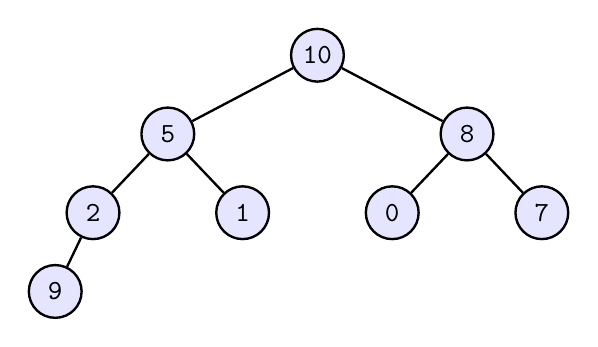
\begin{tikzpicture}

\fill[blue!10] (0.0, 0.0) circle (0.35);
\node [line width=0.03cm,black,minimum size=0.6699999999999999cm,draw,circle] at (0.0,0.0)(10){};\draw (0.0, 0.0) node[color=black] {\texttt{10}};
\fill[blue!10] (-1.9, -1.0) circle (0.35);
\node [line width=0.03cm,black,minimum size=0.6699999999999999cm,draw,circle] at (-1.9,-1.0)(5){};\draw (-1.9, -1.0) node[color=black] {\texttt{5}};
\fill[blue!10] (1.9, -1.0) circle (0.35);
\node [line width=0.03cm,black,minimum size=0.6699999999999999cm,draw,circle] at (1.9,-1.0)(8){};\draw (1.9, -1.0) node[color=black] {\texttt{8}};
\fill[blue!10] (-2.85, -2.0) circle (0.35);
\node [line width=0.03cm,black,minimum size=0.6699999999999999cm,draw,circle] at (-2.85,-2.0)(2){};\draw (-2.85, -2.0) node[color=black] {\texttt{2}};
\fill[blue!10] (-0.95, -2.0) circle (0.35);
\node [line width=0.03cm,black,minimum size=0.6699999999999999cm,draw,circle] at (-0.95,-2.0)(1){};\draw (-0.95, -2.0) node[color=black] {\texttt{1}};
\fill[blue!10] (0.95, -2.0) circle (0.35);
\node [line width=0.03cm,black,minimum size=0.6699999999999999cm,draw,circle] at (0.95,-2.0)(0){};\draw (0.95, -2.0) node[color=black] {\texttt{0}};
\fill[blue!10] (2.85, -2.0) circle (0.35);
\node [line width=0.03cm,black,minimum size=0.6699999999999999cm,draw,circle] at (2.85,-2.0)(7){};\draw (2.85, -2.0) node[color=black] {\texttt{7}};
\fill[blue!10] (-3.33, -3.0) circle (0.35);
\node [line width=0.03cm,black,minimum size=0.6699999999999999cm,draw,circle] at (-3.33,-3.0)(9){};\draw (-3.33, -3.0) node[color=black] {\texttt{9}};\draw[line width=0.03cm,black] (10) to  (5);
\draw[line width=0.03cm,black] (10) to  (8);
\draw[line width=0.03cm,black] (5) to  (2);
\draw[line width=0.03cm,black] (5) to  (1);
\draw[line width=0.03cm,black] (8) to  (0);
\draw[line width=0.03cm,black] (8) to  (7);
\draw[line width=0.03cm,black] (2) to  (9);
\end{tikzpicture}

\end{center}



It's easy to see that in the DFA, the $a$--
and $b$--transitions from the state $\{\}$ goes back to itself.
Therefore the completed DFA is this:


\begin{center}
\begin{tikzpicture}[>=triangle 60,shorten >=0.5pt,node distance=2cm,auto,initial text=, double distance=2pt]
\node[state,initial] (A) at (  0,  0) {$\{q_0\}$};
\node[state] (B) at (  3,  0) {$\{\}$};

\path[->]
(A) edge [bend left=0,pos=0.5,above] node {$a,b$} (B)
(B) edge [loop above] node {$a,b$} ()

;
\end{tikzpicture}
\end{center}
    



\newpage

Solution to Exercise \ref{ex:dfa-as-powerful-as-nfa1}\labeltext{}{sol:dfa-as-powerful-as-nfa1}.

\tinysidebar{\debug{exercises/{dfa-as-powerful-as-nfa1/answer.tex}}}

    Solution not provided.
    

\newpage

Solution to Exercise \ref{ex:dfa-as-powerful-as-nfa2}\labeltext{}{sol:dfa-as-powerful-as-nfa2}.

\tinysidebar{\debug{exercises/{dfa-as-powerful-as-nfa2/answer.tex}}}

    Solution not provided.
    

\newpage

Solution to Exercise \ref{ex:dfa-as-powerful-as-nfa3}\labeltext{}{sol:dfa-as-powerful-as-nfa3}.

\tinysidebar{\debug{exercises/{dfa-as-powerful-as-nfa3/answer.tex}}}

    Solution not provided.
    

\newpage

Solution to Exercise \ref{ex:dfa-as-powerful-as-nfa4}\labeltext{}{sol:dfa-as-powerful-as-nfa4}.

\tinysidebar{\debug{exercises/{dfa-as-powerful-as-nfa4/answer.tex}}}

    Solution not provided.
    

\newpage

Solution to Exercise \ref{ex:closure0}\labeltext{}{sol:closure0}.

\tinysidebar{\debug{exercises/{closure0/answer.tex}}}

    Solution not provided.
    

\newpage

Solution to Exercise \ref{ex:closure1}\labeltext{}{sol:closure1}.

\tinysidebar{\debug{exercises/{closure1/answer.tex}}}

    Solution not provided.
    

\newpage

Solution to Exercise \ref{ex:closure2}\labeltext{}{sol:closure2}.

\tinysidebar{\debug{exercises/{closure2/answer.tex}}}

    Solution not provided.
    

\newpage

Solution to Exercise \ref{ex:closure3}\labeltext{}{sol:closure3}.

\tinysidebar{\debug{exercises/{closure3/answer.tex}}}

    Solution not provided.
    

\newpage

Solution to Exercise \ref{ex:closure4}\labeltext{}{sol:closure4}.

\tinysidebar{\debug{exercises/{closure4/answer.tex}}}

    Solution not provided.
    

\newpage

Solution to Exercise \ref{ex:closure5}\labeltext{}{sol:closure5}.

\tinysidebar{\debug{exercises/{closure5/answer.tex}}}

    Solution not provided.
    

\newpage

Solution to Exercise \ref{ex:closure6}\labeltext{}{sol:closure6}.

\tinysidebar{\debug{exercises/{closure6/answer.tex}}}

    Solution not provided.
    

\newpage

Solution to Exercise \ref{ex:closure7}\labeltext{}{sol:closure7}.

\tinysidebar{\debug{exercises/{closure7/answer.tex}}}

    Solution not provided.
    

\newpage

Solution to Exercise \ref{ex:closure8}\labeltext{}{sol:closure8}.

\tinysidebar{\debug{exercises/{closure8/answer.tex}}}

    Solution not provided.
    

\newpage

Solution to Exercise \ref{ex:closure9}\labeltext{}{sol:closure9}.

\tinysidebar{\debug{exercises/{closure9/answer.tex}}}

    Solution not provided.
    

\newpage

Solution to Exercise \ref{ex:closure10}\labeltext{}{sol:closure10}.

\tinysidebar{\debug{exercises/{closure10/answer.tex}}}

    Solution not provided.
    

\newpage

Solution to Exercise \ref{ex:closure11}\labeltext{}{sol:closure11}.

\tinysidebar{\debug{exercises/{closure11/answer.tex}}}

    Solution not provided.
    

\newpage

Solution to Exercise \ref{ex:closure12}\labeltext{}{sol:closure12}.

\tinysidebar{\debug{exercises/{closure12/answer.tex}}}

    Solution not provided.
    

